\apendice{Documentación de usuario}


\section{Requisitos software y hardware para ejecutar el proyecto.}

\subsection{Software}
El desarrollo de la página web en modo localhost, en lugar de alojarla en un servidor externo, genera unos requerimientos específicos de software. Cumplir con estos requisitos es indespensable para el correcto funcionamiento de la página, asegurando el acceso a esta y permitiendo la comunicación con la base de datos y el Bluetooth del dispositivo hardware.\\

Descripción de los elementos software necesarios y sus respectivas funciones:
\begin{itemize}
    \item XAMPP. Es un paquete de software que a través de su panel de control va a permitir iniciar Apache (servidor web) y MySQL (servidor de bases de datos).
    \item Node.js. Servidor que se inicia desde los comandos de cmd y forma parte del backend para el control de la comunicación entre la web, Arduino y la base de datos.
    \item Scripts y archivos de \textit{Web\_VisualStudio}. Es imprescindible que estén localizados dentro de la carpeta htdocs de XAMPP.
    \item Visual Studio Code. Para ejecutar el archivo \textit{/bluetooth/ArduinoBridge \\ /bridge.py}, puente para la comunicación entre el dispositivo Arduino y el servidor web.
\end{itemize}

Además del software que permite el funcionamiento de la web, es indispensable cargar el script correcto en el microprocesador Arduino:
\begin{itemize}
    \item \textit{version 4.0/v4.0\_solicitudBD.ino}. Una vez el código ha sido compilado y almacenado en el microprocesador no será necesario realizar esta operación más veces, es decir, el usuario final no debería realizar este proceso ya que el hardware estaría configurado de fábrica.
    \item Arduino IDE. Necesario para realizar la subida del script.
    \item Antes de cualquier uso del prototipo hay que cargar y ejecutar el archivo MPU6050-lcd16\_ic2/MPU6050-lcd16\_ic2.ino para su calibración \cite{saragonz91:online}. Esta acción debería realizarse en fábrica, antes de la distribución al usuario final. 
\end{itemize}

Para el correcto funcionamiento de todos los softwares mencionados, se requiere la instalación de una variedad de paquetes y librerías de Arduino, python y Node.js.
\begin{itemize}
    \item Librerías de Arduino: I2Cdev, MPU6050, Wire, SoftwareSerial y LiquidCrystal\_I2C.
    \item Paquetes Pyton: PySerial, Requests.
    \item Paquetes Node.js: Express, MySQL, Body-Parser y CORS.
\end{itemize}

Se procede a la descripción detallada mediante tablas, de los requisitos funcionales específicos del proyecto software que se desarrolla. Van desde la Tabla RF-01 (Tabla \ref{RF-01}) hasta la Tabla RF-08 (Tabla \ref{RF-08}) e incluyen información del funcionamiento de la web y las interacciones con los usuarios.

\begin{table}[p]
    \centering
    \begin{tabularx}{\linewidth}{ p{0.21\columnwidth} p{0.71\columnwidth} }
        \toprule
        \textbf{RF-01}    & \textbf{Iniciar sesión}\\
        \toprule
        \textbf{Descripción}              & Todos los usuarios deben introducir de forma obligatoria su correo electrónico, tipo de usuario y contraseña para poder acceder a la página web.   \\
        \textbf{Importancia}                & Baja \\
        \bottomrule
    \end{tabularx}
    \caption{RF-01 Iniciar Sesión}
    \label{RF-01}
\end{table}

\begin{table}[p]
    \centering
    \begin{tabularx}{\linewidth}{ p{0.21\columnwidth} p{0.71\columnwidth} }
        \toprule
        \textbf{RF-02}    & \textbf{Consultar pacientes y usuarios}\\
        \toprule
        \textbf{Descripción}              & Otorgar acceso a la lista completa de usuarios o pacientes, según los permisos asignados al usuario, y permitir la realización de búsquedas específicas dentro de ella.   \\
        \textbf{Importancia}                & Media \\
        \bottomrule
    \end{tabularx}
    \caption{RF-02 Consultar pacientes y usuarios}
    \label{RF-02}
\end{table}

\begin{table}[p]
    \centering
    \begin{tabularx}{\linewidth}{ p{0.21\columnwidth} p{0.71\columnwidth} }
        \toprule
        \textbf{RF-03}    & \textbf{Gestionar pacientes y usuarios}\\
        \toprule
        \textbf{Descripción}              & Permitir la creación y eliminación de cuentas, así como la modificación de los datos almacenados en las cuentas de pacientes y médicos. La capacidad para realizar estas acciones depende del nivel de acceso que el usuario tenga en el sistema web.   \\
        \textbf{Importancia}                & Media \\
        \bottomrule
    \end{tabularx}
    \caption{RF-03 Gestionar pacientes y usuarios}
    \label{RF-03}
\end{table}

\begin{table}[p]
    \centering
    \begin{tabularx}{\linewidth}{ p{0.21\columnwidth} p{0.71\columnwidth} }
        \toprule
        \textbf{RF-04}    & \textbf{Realizar actividad}\\
        \toprule
        \textbf{Descripción}              & Ofrece las opciones de iniciar y finalizar actividades, así como la opción de guardar o descartar estas mismas.   \\
        \textbf{Importancia}                & Alta \\
        \bottomrule
    \end{tabularx}
    \caption{RF-04 Realizar actividad}
    \label{RF-04}
\end{table}

\begin{table}[p]
    \centering
    \begin{tabularx}{\linewidth}{ p{0.21\columnwidth} p{0.71\columnwidth} }
        \toprule
        \textbf{RF-05}    & \textbf{Mostrar actividades}\\
        \toprule
        \textbf{Descripción}              & Presenta al usuario en una lista las actividades realizadas por el paciente, permitiendo diferentes visualizaciones y llevar a cabo filtrados.   \\
        \textbf{Importancia}                & Alta \\
        \bottomrule
    \end{tabularx}
    \caption{RF-05 Mostrar actividades}
    \label{RF-05}
\end{table}

\begin{table}[p]
    \centering
    \begin{tabularx}{\linewidth}{ p{0.21\columnwidth} p{0.71\columnwidth} }
        \toprule
        \textbf{RF-06}    & \textbf{Consultar estadísticas}\\
        \toprule
        \textbf{Descripción}              & Visualización de los datos relacionados con las actividades realizadas por el paciente, ya sea de una actividad en concreto o de todas en conjunto.   \\
        \textbf{Importancia}                & Media \\
        \bottomrule
    \end{tabularx}
    \caption{RF-06 Consultar Estadísticas}
    \label{RF-06}
\end{table}

\begin{table}[p]
    \centering
    \begin{tabularx}{\linewidth}{ p{0.21\columnwidth} p{0.71\columnwidth} }
        \toprule
        \textbf{RF-07}    & \textbf{Gestionar cuenta}\\
        \toprule
        \textbf{Descripción}              & Facilitar a los usuarios las tareas de cambio de contraseña y actualización del correo eléctrónico vinculado a su cuenta.  \\
        \textbf{Importancia}                & Baja \\
        \bottomrule
    \end{tabularx}
    \caption{RF-07 Gestionar cuenta}
    \label{RF-07}
\end{table}

\begin{table}[p]
    \centering
    \begin{tabularx}{\linewidth}{ p{0.21\columnwidth} p{0.71\columnwidth} }
        \toprule
        \textbf{RF-08}    & \textbf{Cerrar sesión}\\
        \toprule
        \textbf{Descripción}              & Todos los usuarios tendrán la opción de cerrar sesión desde el menú de inicio. Para prevenir cierres accidentales, se solicitará una confirmación de la acción antes de que esta se complete.  \\
        \textbf{Importancia}                & Baja \\
        \bottomrule
    \end{tabularx}
    \caption{RF-08 Cerrar sesión}
    \label{RF-08}
\end{table}

\subsection{Hardware}
El funcionamiento correcto de todo el proyecto requiere del dispositivo físico adecuado que trabaje en concordancia con el software desarrollado, fin con el que se han realizado cambios y adiciones de componentes sobre el hardware del prototipo inicial. En la Tabla \ref{tab:componentes} se muestran todos los componentes empleados.

\begin{table}[]
    \begin{tabular}{|c|c|}
    \hline
    \rowcolor[HTML]{FFFFFF} 
    \multicolumn{2}{|c|}{\cellcolor[HTML]{FFFFFF}\textbf{Componentes}} \\ \hline 
    \rowcolor[HTML]{EFEFEF} 
    Arduino UNO R3 & 2 Resistencias \\ \hline
    \rowcolor[HTML]{FFFFFF} 
    Display LCD + Interfaz I2C & 2 Pulsadores \\ \hline
    \rowcolor[HTML]{EFEFEF} 
    Bluetooth HC-05 & Sensor MPU-6050 \\ \hline
    \rowcolor[HTML]{FFFFFF} 
    Cables & Caja para Prototipos \\ \hline
    \rowcolor[HTML]{EFEFEF} 
    Batería Recargable 9V + Conector de Batería & Cable Multihilo Flexible \\ \hline
    \rowcolor[HTML]{FFFFFF} 
    Proto Shield Arduino & Interruptor \\ \hline
    \rowcolor[HTML]{EFEFEF} 
    Conector 5 pines macho-hembra & \\ \hline
    \end{tabular}
    \caption{Componentes del Prototipo}
    \label{tab:componentes}
\end{table}



Los requisitos hardware se basan en el principal elemento que da pie a este proyecto, el Bluetooth, y en la necesidad de implementar mejoras para lograr una mayor facilidad de uso y comodidad. Su descripción se incluye en las tablas RF-09 ( Tabla \ref{RF-09}) a RF-12 (Tabla \ref{RF-12}).

\begin{table}[p]
    \centering
    \begin{tabularx}{\linewidth}{ p{0.21\columnwidth} p{0.71\columnwidth} }
        \toprule
        \textbf{RF-09}    & \textbf{Transmisión de datos sin cables}\\
        \toprule
        \textbf{Descripción}              & Implementación de la tecnología de comunicación escogida para que el envío de datos del dispositivo no dependa de la conexión por USB al ordenador.  \\
        \textbf{Importancia}                & Alta \\
        \bottomrule
    \end{tabularx}
    \caption{RF-09 Transmisión de datos sin cables}
    \label{RF-09}
\end{table}

\begin{table}[p]
    \centering
    \begin{tabularx}{\linewidth}{ p{0.21\columnwidth} p{0.71\columnwidth} }
        \toprule
        \textbf{RF-10}    & \textbf{Alimentación externa}\\
        \toprule
        \textbf{Descripción}              & Permitir la completa autonomía del prototipo incorporando en él una batería externa recargable. \\
        \textbf{Importancia}                & Alta \\
        \bottomrule
    \end{tabularx}
    \caption{RF-10 Alimentación externa}
    \label{RF-10}
\end{table}

\begin{table}[p]
    \centering
    \begin{tabularx}{\linewidth}{ p{0.21\columnwidth} p{0.71\columnwidth} }
        \toprule
        \textbf{RF-11}    & \textbf{Encendido y apagado del sistema}\\
        \toprule
        \textbf{Descripción}              & Regulación del flujo eléctrico que recibe el sistema. Se puede lograr de forma sencilla a través de un interruptor. \\
        \textbf{Importancia}                & Media \\
        \bottomrule
    \end{tabularx}
    \caption{RF-11 Encendido y apagado del sistema}
    \label{RF-11}
\end{table}

\begin{table}[p]
    \centering
    \begin{tabularx}{\linewidth}{ p{0.21\columnwidth} p{0.71\columnwidth} }
        \toprule
        \textbf{RF-12}    & \textbf{Seguridad y manejabilidad del prototipo}\\
        \toprule
        \textbf{Descripción}              & Es imprescindible, tanto para la protección del prototipo como para la seguridad del usuario, que el hardware y el montaje electrónico se encuentren protegidos y aislados. La solución que se implemente debe asegurar un manejo sencillo del dispositivo.  \\
        \textbf{Importancia}                & Alta \\
        \bottomrule
    \end{tabularx}
    \caption{RF-12 Seguridad y manejabilidad del prototipo}
    \label{RF-12}
\end{table}


\section{Instalación / Puesta en marcha}
Esta sección proporciona una guía detallada para que cualquier usuario pueda instalar y comenzar a utilizar el producto final de este proyecto. Se explican los procedimientos necesarios para la preparación del dispositivo y el despliegue de la web.

Antes de inicar cualquier proceso detallado en esta sección, es imprescindible tener instalados y configurados correctamente los siguientes programas software con sus respectivas librerías y paquetes: VS Code, Node.js, XAMPP y Arduino IDE. Para más información detallada, consultar el anexo \textit{B.1. Requisitos software y hardware para ejecutar el proyecto} y el apartado \textit{4.2. Técnicas y herramientas} de la memoria.

\subsection{Configuración del dispositivo}
\begin{enumerate}
    \item Proceso de calibración. Abrir el archivo \textit{Arduino/version 4.0/v4.0\_soli-\\citudBD/v4.0\_solicitudBD.ino} y realizar carga del programa en la placa Arduino. Una vez completada la carga, se debe abrir el monitor serial, asegurándose que esté configurado para una velocidad de transmición de 115200 baudios. Para completar con éxito el proceso de calibración, el usuario debe seguir todas las instrucciones que aparecen en el monitor serial. La Figura \ref{fig:calibrado} muestra el ejemplo de un proceso de calibración adecuado, en el que los offsets presentan valores similares a la referencia.
    \begin{figure}[h]
        \centering
        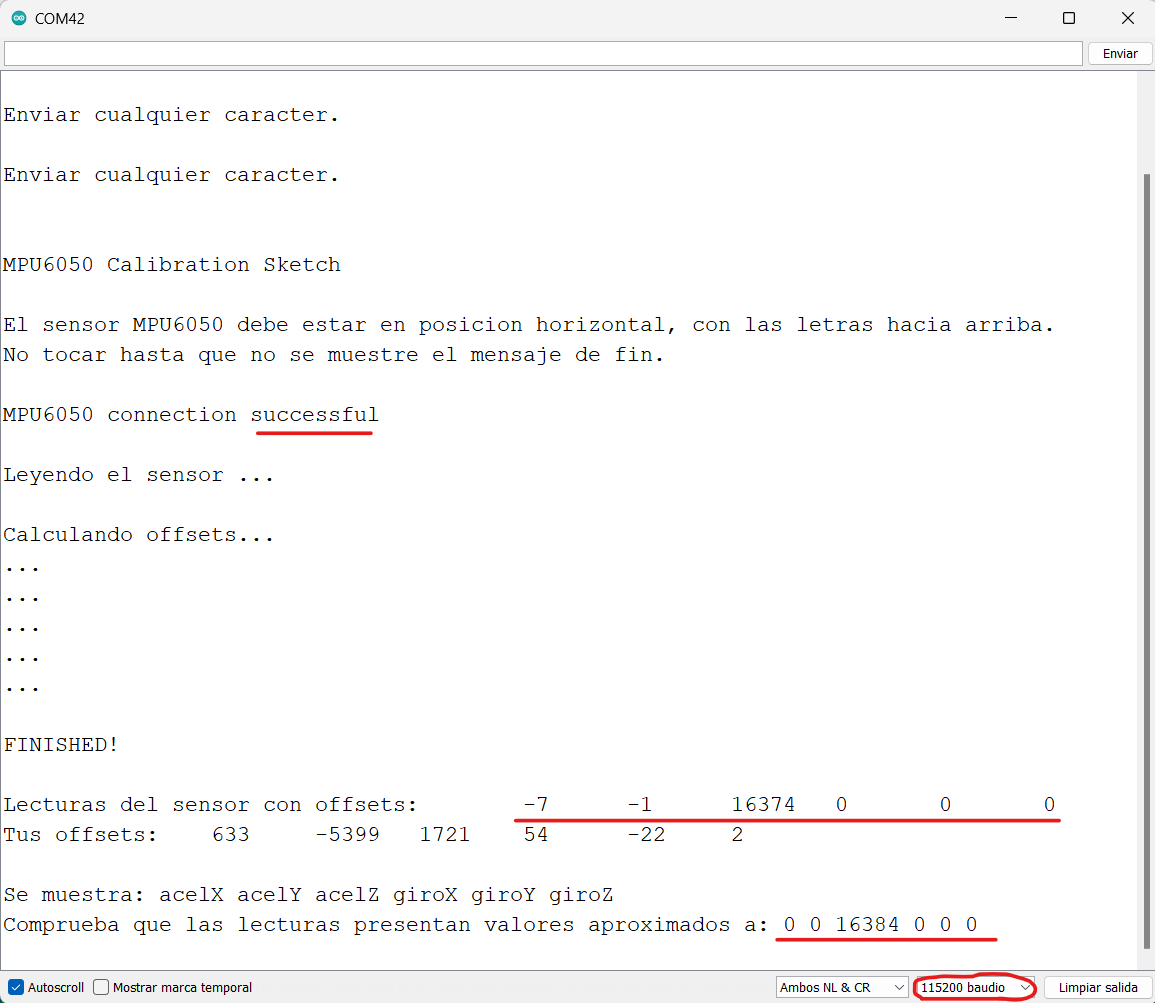
\includegraphics[width=1\textwidth]{img/B2_InstalacionPuestaMarcha/calibrado_subrayado.png}
        \caption{Proceso de calibrado.}
        \label{fig:calibrado}
    \end{figure}
    
    \item Carga del programa principal. Realizar la subida del archivo \textit{Arduino/version 4.0/v4.0\_solicitudBD/v4.0\_solicitudBD.ino} desde Arduino IDE a la placa de Arduino.
\end{enumerate}

\subsection{Despliegue de la aplicación web en entorno local}
\begin{enumerate}
    \item Acciones necesarias con XAMPP.\\
    Únicamente es necesario seguir los pasos a continuación descritos, la primera vez que se descargan los archivos y se quiere desplegar la web.
    \begin{enumerate}
        \item Incluir la carpeta \textit{Web\_VisualStudio/} en el directorio \textit{xampp/htdocs} del equipo. La localización de dicho directorio puede variar según lo seleccionado durante el proceso de instalación. El repositorio de \href{https://github.com/imb1006/Web_Seguimiento_Parkinson}{GitHub} del proyecto contiene el archivo \textit{Web\_VisualStudio.zip} para facilitar la descarga.
        
        \item Iniciar Apache y MySQL desde XAMPP Control Panel (Figura \ref{fig:xampp}). Este paso sí se va a tener que realizar siempre que se quiera utilizar la plataforma web.
            \begin{figure}[h]
                \centering
                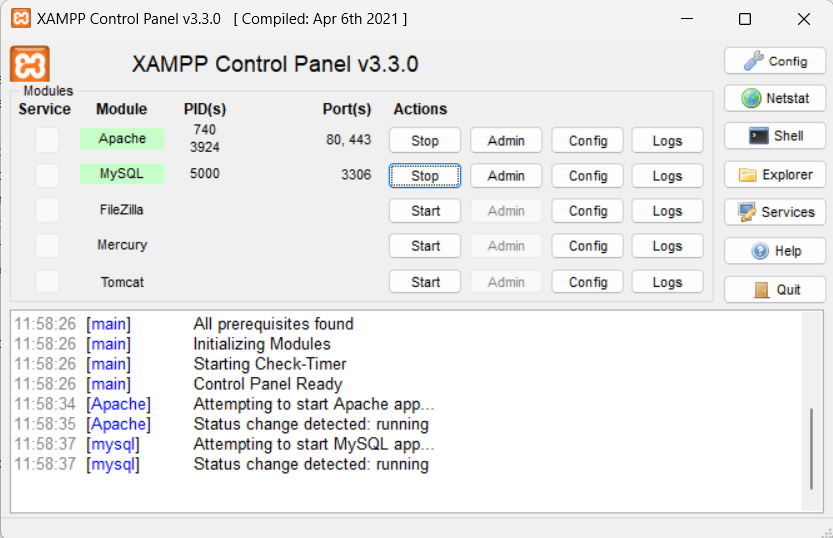
\includegraphics[width=1\textwidth]{img/B2_InstalacionPuestaMarcha/xampp.png}
                \caption{XAMPP Control Panel.}
                \label{fig:xampp}
            \end{figure}
            
        \item Crear la base de datos. Para realizar este proceso se debe navegar a la dirección \textit{localhost/phpmyadmin}, crear una nueva base de datos bajo el nombre 'WebParkinson' e importar el archivo \textit{DataBase/DataBase.sql}.
    \end{enumerate}
    
    \item Iniciar el servidor. El usuario debe dirigirse al directorio \textit{bluetooth/Ard-\\uinoServer/} y, una vez entre en él, debe abrir el terminal de comandos (cdm) haciendo clic derecho y seleccionando la opción correspondiente. Dentro del terminal, ejecutar el comando 'node server.js'. Si el proceso se realiza correctamente, aparecerá un mensaje similar al mostrado en la Figura \ref{fig:server}. En caso de que no se haya instalado MySQL en el servidor, se mostrará un mensaje de error y se deberá proceder a ejecutar el comando 'npm install mysql', tal y como se indica en la Figura \ref{fig:mysql}.

    \begin{figure}[h]
        \centering
        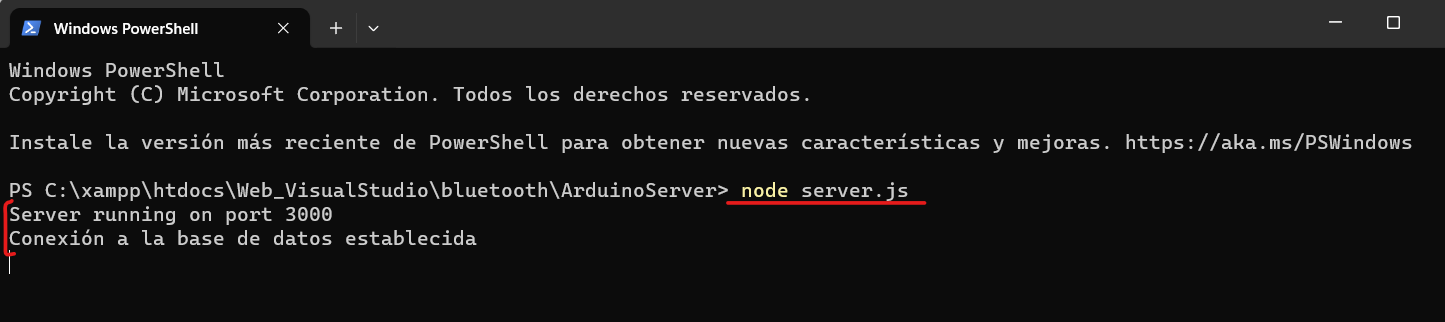
\includegraphics[width=1\textwidth]{img/B2_InstalacionPuestaMarcha/server_subrayado.png}
        \caption{Éxito en la inicialización del servidor.}
        \label{fig:server}
    \end{figure}

    \begin{figure}[h]
        \centering
        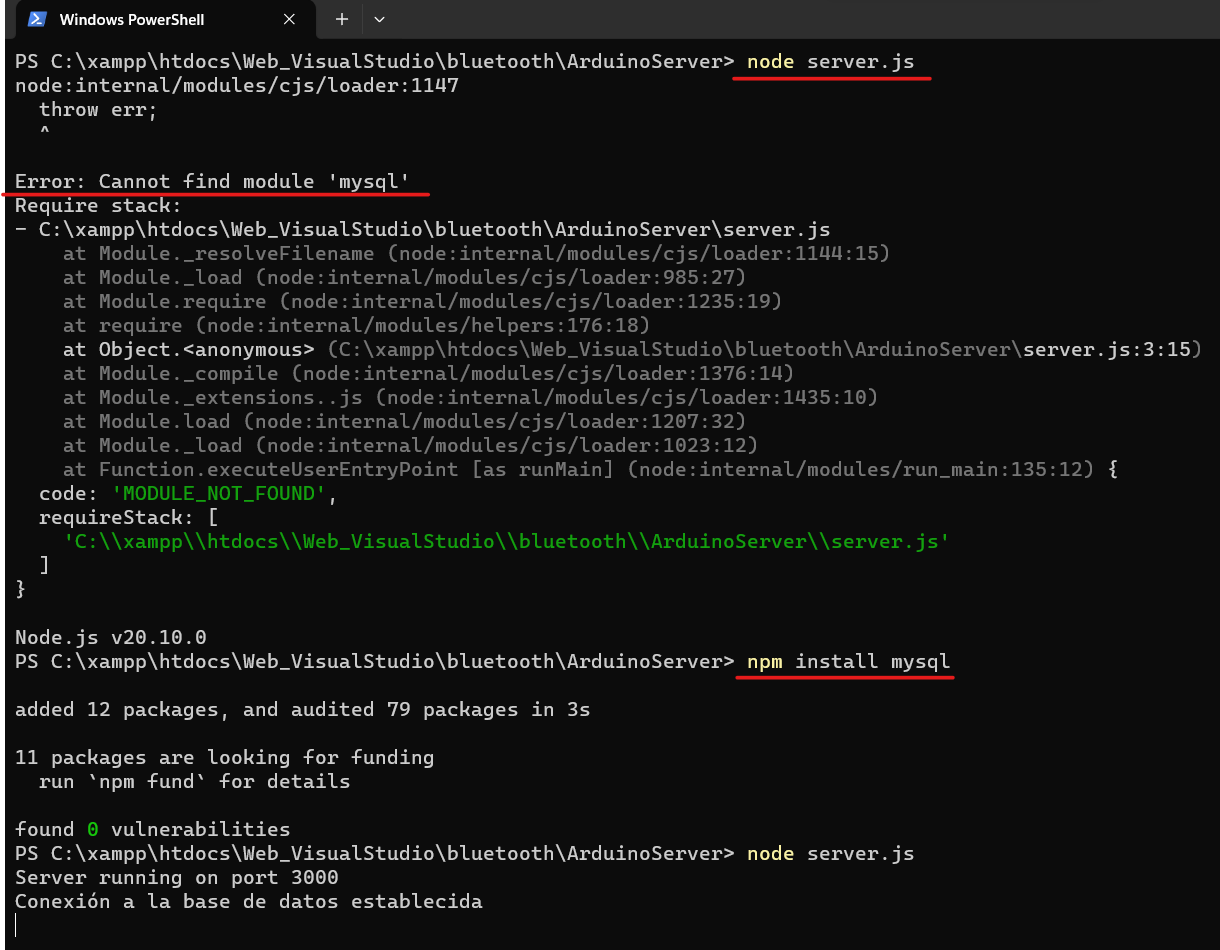
\includegraphics[width=1\textwidth]{img/B2_InstalacionPuestaMarcha/mysql_subrayado.png}
        \caption{Instalación de MySQL en el servidor.}
        \label{fig:mysql}
    \end{figure}
    
    \item Ejecutar \textit{bluetooth/ArduinoBridge/bridge.py}. La ejecución se debe realizar desde VS Code. Es importante verificar siempre el número del puerto COM asignado al Bluetooth, porque puede variar y entonces será necesario modificar el script (Figura \ref{fig:com}). En el 'Administrador de dispositivos' de Windows se puede observar el número de puerto.
    \begin{figure}[h]
        \centering
        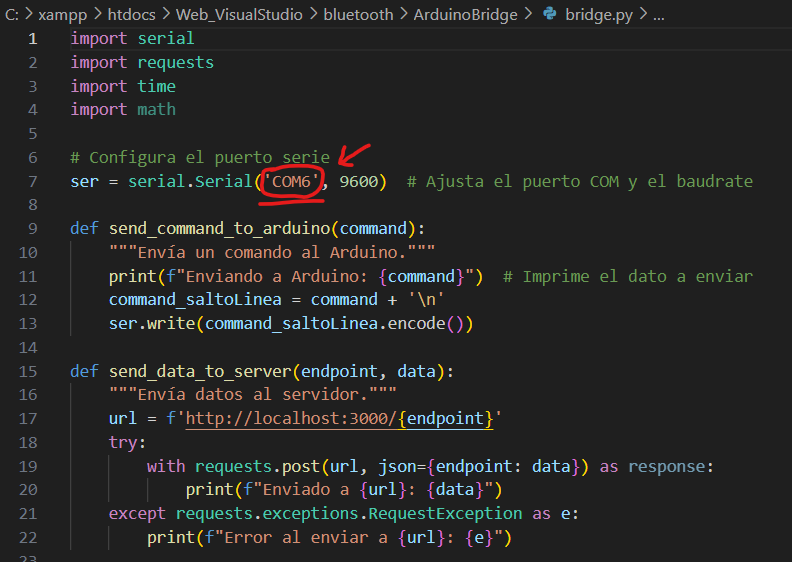
\includegraphics[width=1\textwidth]{img/B2_InstalacionPuestaMarcha/com.png}
        \caption{Fragmento del script \textit{bridge.py} en el que se debe modificar el puerto COM.}
        \label{fig:com}
    \end{figure}
    
\end{enumerate}


\section{Manuales y/o Demostraciones prácticas}




    
     